\section{Análise Exploratória}

A Análise Exploratória de Dados (AED) é uma etapa do fluxo de aprendizado de máquina que permite realizar uma exploração dos dados baseada em técnicas da Estatística Descritiva. Para essa etapa da pesquisa foi utilizado o notebook \textbf{analise-exploratoria.ipynb}. Por se tratar de uma atividade interativa, a utilização de um Jupyter Notebook se mostrou mais eficiente do que a utilização direta de um script Python.

Um primeiro aspecto que chamou a atenção na exploração dos dados foi a predominância de Atos Declaratórios Executivos (ADE), representando 71,79\% (14.948 dos 20.821 atos analisados), seguido pelas Soluções de Consulta (SC) com 14,98\% e Portarias (Port.) com 10,60\%. Os demais tipos de ato representam juntos 2.63\% do total. A figura \ref{fig:atos-por-tipo-ato} evidencia essa distribuição:

\begin{figure}[h]
	\caption{Quantidade de Atos por Tipo de Ato}
	\center
	\label{fig:atos-por-tipo-ato}
	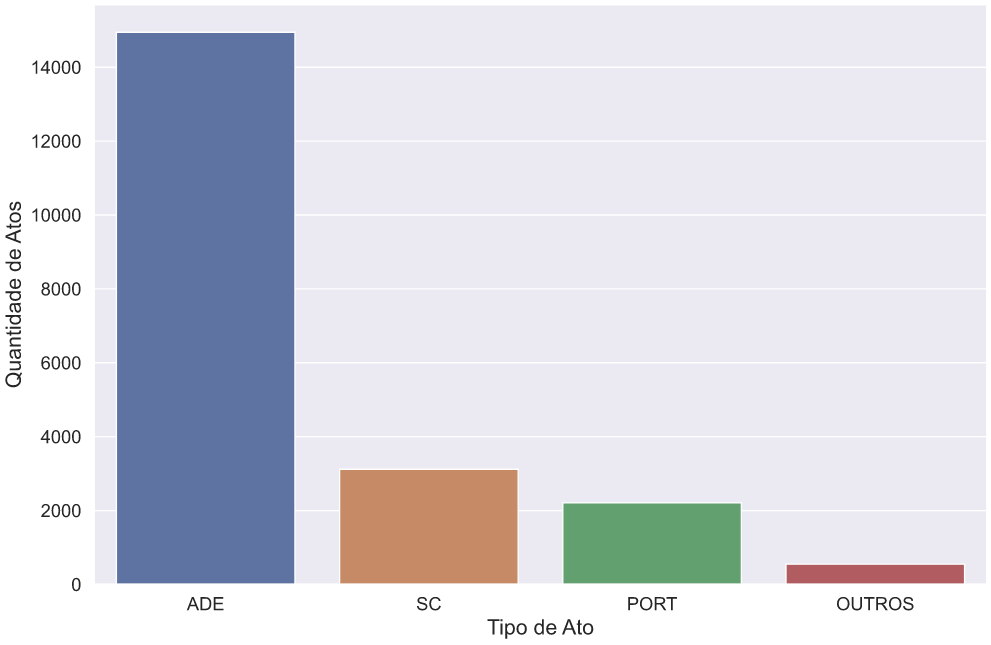
\includegraphics[scale=1.7]{exploratoria/atos-por-tipo-ato.png}
	\fdp
\end{figure}